\section{Evaluation}
% 评估
\label{sec:eval}

Our evaluation addresses two research questions:
% 我们的评估围绕两个研究问题展开：

\begin{itemize}[leftmargin=*]
  \item \textbf{RQ1 (Policy Expression and Benefits):} Can AI agents safely express GPU resource-management policies through \sys---including reimplementations of published state-of-the-art systems---and do those policies improve performance?
  % RQ1（策略表达与收益）：AI 智能体能否通过 gpubpf 安全地表达 GPU 资源管理策略——包括对己发表最先进系统的重实现——这些策略能否提升性能？
  \item \textbf{RQ2 (Mechanism Cost):} What does the \sys{} mechanism cost, in hook and observability overhead and in executing the same policy through \sys{}?
  % RQ2（机制代价）：gpubpf 机制的代价有多大——包括钩子与可观测开销，以及通过 gpubpf 执行同一策略的代价？
\end{itemize}

We answer RQ1 in \S\ref{sec:rq1} through policy microbenchmarks, agent-driven case studies on realistic workloads, multi-tenant settings, and matched reimplementations of published policies. \S\ref{sec:rq2-cost} answers RQ2.
% 我们在 \S\ref{sec:rq1} 通过策略微基准、真实负载上的智能体驱动案例研究、多租户场景，以及对已发表策略的匹配重实现回答 RQ1；\S\ref{sec:rq2-cost} 回答 RQ2。

\subsection{Methodology and Setup}
% 方法论与实验设置

We evaluate \sys on two machines: Server~A with Intel Core Ultra~9 285K (24 cores), 128~GB DDR5 RAM, and NVIDIA RTX~5090 GPU; Server~B with dual Intel Gold 6138 (80 cores), 256~GB RAM, and NVIDIA P40 GPU.
% 我们在两台机器上评估 gpubpf：服务器 A 配备 Intel Core Ultra 9 285K（24 核）、128 GB DDR5 内存和 NVIDIA RTX 5090 GPU；服务器 B 配备双路 Intel Gold 6138（80 核）、256 GB 内存和 NVIDIA P40 GPU。
Unless otherwise specified, experiments run on Server~A, averaging 10 trials using geometric mean.
% 除非另有说明，实验均在服务器 A 上进行，每项结果取 10 次试验的几何平均值。
We compare \sys{} against three classes of baselines: (1) driver defaults (UVM LRU/FIFO eviction, native GPU scheduler), (2) application-level hints (\texttt{cudaMemAdvise}), and (3) framework-managed policies (e.g., llama.cpp \texttt{ncmoe}, vLLM CPU offload, LMCache) where applicable.
% 我们将 gpubpf 与三类基线对比：(1) 驱动默认行为（UVM LRU/FIFO 驱逐、原生 GPU 调度器），(2) 应用层提示（\texttt{cudaMemAdvise}），以及 (3) 框架管理的策略（如 llama.cpp 的 \texttt{ncmoe}、vLLM CPU offload、LMCache，在适用处）。
The matched comparisons in \S\ref{sec:policy-mechanism} additionally evaluate policies from published research systems: MoE-Infinity~\cite{xue2025moeinfinity}, XSched~\cite{shen2025xsched}, GPREEMPT~\cite{fan2025gpreempt}, Expert Buffering~\cite{huang2023towards}, FineMoE~\cite{yu2026finemoe}, Hummingbird~\cite{hu2026hummingbird}, and POD-Attention~\cite{kamath2025pod}; each pairs a native policy implementation with a \sys{} port.
% \S\ref{sec:policy-mechanism} 进一步评估 MoE-Infinity、XSched、GPREEMPT、Expert Buffering、FineMoE、Hummingbird 和 POD-Attention 等已发表系统的策略；每组配对原生策略实现和 \sys{} 移植版。
We use PyTorch (version 2.9.0) and vLLM (version 0.11.0) with custom allocators, llama.cpp (version 7101), and Faiss (version 1.13.0) with UVM build config.
% 我们使用 PyTorch（版本 2.9.0）和 vLLM（版本 0.11.0，配自定义分配器）、llama.cpp（版本 7101）以及采用 UVM 构建配置的 Faiss（版本 1.13.0）。
Driver-attached \sys{} policies can operate without application-source changes; the matched research-policy ports and storage-tier comparison use the adapters and shared executors described below.
% 驱动挂接的 \sys{} 策略可以无需修改应用源码运行；匹配的研究策略移植和存储层对比则使用下文说明的适配器与共享执行器。

\begin{figure}
\centering

\includegraphics[width=\columnwidth]{img/results-raw/clc/microbench_combined.pdf}
\caption{Single-tenant policy evaluation (normalized speedup, higher is better): (a) memory prefetch policies on vector-add; (b) block scheduling policies on GEMM.}
% 单租户策略评估（归一化加速比，越高越好）：(a) vector-add 上的内存预取策略；(b) GEMM 上的块调度策略。
\label{fig:clc-policies}

\end{figure}

\subsection{RQ1: Policy Expression and Benefits}
% RQ1：策略表达与收益
\label{sec:rq1}

\subsubsection{Single-Tenant Memory and Scheduling Policies}
% 单租户内存与调度策略
\label{sec:rq1-micro}

\paragraph{Memory Prefetch Policies.}
% 内存预取策略。
We evaluate host-device prefetch coordination using a vector-add GPU kernel~\cite{nvidia_cuda_samples} with stride access pattern and 40GB working set (1.25$\times$ oversubscription).
% 我们使用具有步长访问模式、40GB 工作集（1.25× 超订）的 vector-add GPU 内核~\cite{nvidia_cuda_samples}评估主机—设备预取协同。
Device-side L2 prefetch instructions (\texttt{prefetch.\allowbreak{}global.\allowbreak{}L2}) trigger non-blocking page faults, while host-side callbacks extend prefetching to additional pages.
% 设备端 L2 预取指令（\texttt{prefetch.\allowbreak{}global.\allowbreak{}L2}）触发非阻塞缺页，而主机端回调将预取扩展到更多页面。
As shown in \Cref{fig:clc-policies}a, device-only prefetch at thread entry achieves 1.34$\times$ speedup while combined host-device stride-based eBPF prefetch achieves 1.77$\times$.
% 如 \Cref{fig:clc-policies}a 所示，仅设备端预取在线程入口处取得 1.34× 加速，而主机—设备协同的步长式 eBPF 预取达到 1.77×。
However, sequential prefetch degrades performance by 8\% due to pattern mismatch.
% 然而，顺序预取因模式不匹配导致性能下降 8\%。

\paragraph{Single-Tenant Block Scheduler.}
% 单租户块调度器。
We apply a \sys-based thread block scheduler to workloads with load imbalance.
% 我们将基于 gpubpf 的线程块调度器应用于存在负载不均衡的工作负载。
Using cluster-style launch where persistent worker blocks pull work units through a policy decision, we evaluate three policies: FixedWork (static block assignment, no scheduler), Greedy (always-steal), and LatencyBudget (workload-aware with per-block time limits).
% 采用集群式启动，由持久工作块根据策略决策 拉取工作单元，我们评估三种策略：FixedWork（静态块分配，无调度器）、Greedy（总是窃取）和 LatencyBudget（感知负载、带每块时间限制的策略）。
\Cref{fig:clc-policies}b compares these policies across two GEMM workloads.
% \Cref{fig:clc-policies}b 在两种 GEMM 工作负载上对比了这些策略。
Under moderate imbalance, both Greedy and LatencyBudget reduce latency by $\sim$11\%.
% 在中等不均衡下，Greedy 和 LatencyBudget 均将延迟降低约 11\%。
Under heavy-tail workloads where 10\% of blocks perform 100--200$\times$ more work, Greedy increases latency by 20\% due to contention on heavy blocks.
% 在 10\% 的块承担 100--200× 更多工作量的重尾负载下，Greedy 因对重块的竞争使延迟增加 20\%。
LatencyBudget, which caps per-block stealing time, matches fixed-work baseline.
% LatencyBudget 限制了每块的窃取时间，与固定分配基线持平。
This highlights \sys's programmability: different workloads require different scheduling strategies.
% 这凸显了 gpubpf 的可编程性：不同工作负载需要不同的调度策略。

\subsubsection{Agent-Driven Policy Exploration Case Studies}
% 智能体驱动的策略探索案例研究
\label{sec:rq1-agent}

We provided an AI coding agent (Claude Code with Opus 4.5) with \sys{}'s eBPF interfaces; the agent autonomously generated all policy logic without human review or guidance, while humans authored only the initial framework and benchmark harness.
% 我们向一个 AI 编程智能体（Claude Code，Opus 4.5）提供 gpubpf 的 eBPF 接口；智能体在无人审阅或指导的情况下自主生成了全部策略逻辑，人类只编写初始框架和基准测试工具。
All 59 policies evaluated were produced via a fully automated generate-test-iterate loop.
% 评估的全部 59 个策略均由完全自动化的“生成—测试—迭代”循环产出。
We conclude with four case studies showing performance gains and the exploration process.
% 最后我们通过四个案例研究展示性能收益与探索过程。

\paragraph{Expert Offloading (llama.cpp GPT-OSS-120B).}
% 专家卸载（llama.cpp GPT-OSS-120B）。
We evaluate \sys on GPT-OSS-120B MXFP4 MoE (59~GB) in llama.cpp on RTX 5090 (32~GB), requiring 1.84$\times$ oversubscription.
% 我们在 RTX 5090（32 GB）上的 llama.cpp 中评估 GPT-OSS-120B MXFP4 MoE（59 GB），需要 1.84× 超订。
We compare five configurations: framework-managed CPU offloading (\texttt{ncmoe=\allowbreak{}32/64}), default UVM, UVM with application-level hints (\texttt{cuda\-Mem\-Advise}), and \sys with eBPF-based host-device prefetching (\S\ref{sec:design-interfaces}).
% 我们对比五种配置：框架管理的 CPU 卸载（\texttt{ncmoe=\allowbreak{}32/64}）、默认 UVM、带应用层提示的 UVM（\texttt{cuda\-Mem\-Advise}），以及采用基于 eBPF 的主机—设备预取的 gpubpf（\S\ref{sec:design-interfaces}）。
\Cref{fig:llama-expert-offload} shows prefill and decode throughput.
% \Cref{fig:llama-expert-offload} 给出了预填充与解码吞吐量。
For decode (memory-bound), \sys achieves \textbf{1.76$\times$ speedup} over application-tuned UVM hints (\texttt{cuda\-Mem\-Advise}) and 4.8$\times$ over framework offloading (\texttt{ncmoe=64}).
% 对于解码（内存受限），gpubpf 相比经应用调优的 UVM 提示（\texttt{cuda\-Mem\-Advise}）取得 \textbf{1.76× 加速}，相比框架卸载（\texttt{ncmoe=64}）取得 4.8× 加速。
This is a policy gain over baseline policies; \S\ref{sec:policy-mechanism} separately measures the cost of executing the same policy through \sys{}.
% 这是相对基线策略的策略收益；\S\ref{sec:policy-mechanism} 单独测量了通过 gpubpf 执行同一策略的代价。
These hints improve decode over default UVM but require application modification and degrade prefill by 40\%; \sys outperforms hints on decode while preserving prefill within 4\% of default UVM, without application changes.
% 这些提示相比默认 UVM 改善了解码，但需要修改应用，并使预填充性能下降 40\%；gpubpf 在解码上优于提示，同时将预填充保持在默认 UVM 的 4\% 以内，且无需修改应用。
For prefill (compute-bound), framework offloading (\texttt{ncmoe=32}) achieves 13\% higher prefill throughput than \sys{}, but decode dominates end-to-end latency, so the decode improvement outweighs the prefill gap.%\arq{I don't understand the final data point. what has 13\% higher throughput? The graphed performance of UVM eBPF looks like it has worse performance compared to the alternatives. BTW---its very weird that none of the bars in Figure 8 are labeled "\sys"--I think that UVM eBPF is supposed to be that configuration but it does not make a lot of sense.}
% 对于预填充（计算受限），框架卸载（\texttt{ncmoe=32}）比 gpubpf 的预填充吞吐量高 13\%，但解码主导端到端延迟，因此解码的改善超过了预填充的差距。

The agent arrived at the final policy through iterative exploration: sequential prefetch degraded decode throughput due to mismatch with MoE stride patterns (consistent with the 8\% degradation in \Cref{fig:clc-policies}a), leading to stride-based prefetch aligned with regular weight layout within each expert layer.
% 智能体通过迭代探索得出最终策略：顺序预取因与 MoE 步长模式不匹配而降低了解码吞吐量（与 \Cref{fig:clc-policies}a 中 8\% 的下降一致），于是改为与各专家层内规则权重布局对齐的步长预取。
Device-side eBPF tracing of per-warp memory accesses revealed that expert activations follow predictable stride sequences and identified frequently-accessed shared layers.
% 对每 warp 内存访问的设备端 eBPF 追踪表明，专家激活遵循可预测的步长序列，并识别出被频繁访问的共享层。
For eviction, the agent tested FIFO ordering before converging on LFU, which retains frequently-accessed shared layers while evicting cold expert pages.
% 在驱逐方面，智能体先测试 FIFO 顺序，最终收敛到 LFU——它保留被频繁访问的共享层，同时驱逐冷的专家页面。
The final policy combines device-side access observation, host-side stride prefetch, and LFU eviction (\S\ref{sec:design-interfaces}).
% 最终策略结合了设备端访问观测、主机端步长预取和 LFU 驱逐（\S\ref{sec:design-interfaces}）。

% \xiangyu{Are those hints easy to find in many scenarios? Maybe we should clarify it. Otherwise, it seems that \sys{} uses some tricks to win the competition.}

\begin{figure}
\centering

\includegraphics[width=\columnwidth]{img/results-raw/llama.cpp/llama_uvm_combined_color.pdf}

\caption{Prefill and decode throughput for GPT-OSS-120B MoE on llama.cpp.}
% llama.cpp 上 GPT-OSS-120B MoE 的预填充与解码吞吐量。
\label{fig:llama-expert-offload}

\end{figure}

\paragraph{KV-cache Offloading (vLLM Qwen-30B MoE).}
% KV-cache 卸载（vLLM Qwen-30B MoE）。
We evaluate \sys on the Qwen-30B FP8 MoE model ($\approx$30GB) on RTX 5090 (32GB).
% 我们在 RTX 5090（32GB）上评估 Qwen-30B FP8 MoE 模型（约 30GB）。
The model nearly fills GPU VRAM, so the default no-offload configuration OOMs under load.
% 该模型几乎占满 GPU 显存，因此默认的不卸载配置在负载下会 OOM。
We stress KV-cache growth by sending 100 concurrent requests from ShareGPT~\cite{sharegpt} (single-round, no prefix caching), resulting in 36--40GB total footprint ($\approx$60K tokens KV-cache).
% 我们通过发送来自 ShareGPT~\cite{sharegpt} 的 100 个并发请求（单轮、无前缀缓存）施加 KV-cache 增长压力，总占用达 36--40GB（约 60K token 的 KV-cache）。
Existing solutions offload KV-cache or experts but not both; UVM attempts on-demand migration of both, leading to thrashing.
% 现有方案只卸载 KV-cache 或专家权重之一；UVM 则尝试对二者按需迁移，导致抖动。
We compare vLLM's CPU-offload mode (\texttt{--cpu-offload-gb 8}) against \sys with UVM and a sequential prefetch policy.
% 我们将 vLLM 的 CPU 卸载模式（\texttt{--cpu-offload-gb 8}）与采用 UVM 和顺序预取策略的 gpubpf 进行对比。
\sys improves mean and p99 time-to-first-token by 1.7--2$\times$ and decoding throughput by 1.3$\times$ over vLLM's default framework-managed offload (\Cref{fig:vllm-kv-offload}), matching LMCache~\cite{lmcache}, a state-of-the-art KV-cache offloading framework.
% 相比 vLLM 默认的框架管理卸载，gpubpf 将平均和 p99 首 token 时间改善 1.7--2×，解码吞吐量提高 1.3×（\Cref{fig:vllm-kv-offload}），与最先进的 KV-cache 卸载框架 LMCache~\cite{lmcache} 持平。
Notably, UVM without \sys policies performs worse than vLLM's offload, while \sys performs similarly to the best framework offloading, with better tail latency, dynamically and transparently.
% 值得注意的是，没有 gpubpf 策略的 UVM 表现不如 vLLM 的卸载，而 gpubpf 以动态、透明的方式达到了与最佳框架卸载相当的效果，且尾延迟更优。

Under memory pressure, the main challenge is managing two competing data types: KV-cache, exhibiting temporal locality (recent tokens accessed frequently during attention) and per-request spatial locality, and model weights with stride patterns in matrix operations.
% 在内存压力下，主要挑战是管理两类相互竞争的数据：具有时间局部性（最近的 token 在注意力计算中被频繁访问）和每请求空间局部性的 KV-cache，以及在矩阵运算中具有步长模式的模型权重。
A uniform sequential prefetch initially caused mutual thrashing between KV-cache and weight pages.
% 统一的顺序预取最初导致 KV-cache 与权重页面之间相互抖动。
Using device-side tracing, the agent explored region-differentiated prefetch strategies, converging on adaptive aggressiveness guided by PCIe utilization and region type (stride for weights, sequential for KV-cache), coupled with LFU eviction retaining frequently accessed pages.
% 利用设备端追踪，智能体探索了分区域差异化的预取策略，最终收敛到由 PCIe 利用率和区域类型（权重用步长、KV-cache 用顺序）调节的自适应预取强度，并配合 LFU 驱逐保留被频繁访问的页面。
The resulting policy effectively prevents thrashing seen with default LRU.
% 由此得到的策略有效避免了默认 LRU 下的抖动。

\begin{figure}
\centering

\includegraphics[width=\columnwidth]{img/results-raw/vllm/ttft_tpot_combined.pdf}

\caption{Time-to-first-token and decoding throughput on Qwen-30B MoE inference with vLLM.}
% vLLM 上 Qwen-30B MoE 推理的首 token 时间与解码吞吐量。
\label{fig:vllm-kv-offload}

\end{figure}

\paragraph{Storage-tier Policy (LMCache).}
% 存储层策略（LMCache）。
We extend LMCache 0.5.4 with native and driver-BPF admission policies over real cuFile compatibility-mode disk I/O on RTX 5090; this does not establish hardware NVMe-to-GPU P2P.
% 我们在 RTX 5090 上为 LMCache 0.5.4 的真实 cuFile 兼容模式磁盘 I/O 加入原生和驱动 BPF 准入策略；这不代表已实现硬件 NVMe 到 GPU 的 P2P。
Both submit demand reads immediately and defer safe background writes while demand reads remain pending; LMCache performs the transfers, and a shared event-driven executor waits for demand drain or cumulative budget expiry before requesting a fresh decision.
% 两者均立即提交需求读取，在仍有需求读取未完成时延迟可安全推迟的后台写入；LMCache 执行传输，共享事件驱动执行器等待需求读取清空或累计预算到期，再请求新的决策。
Five balanced blocks compare FIFO with native/BPF policies at 10 and 200 ms budgets, each using 64 reads and 96 writes of 24 MiB objects at 2/4 ms arrivals.
% 五个平衡轮次比较 FIFO 与采用 10 和 200 ms 预算的原生/BPF 策略，每次以 2/4 ms 到达间隔执行 64 次读取和 96 次写入，对象大小为 24 MiB。
Increasing the cumulative budget from 10 to 200 ms lowers BPF read p99 by a paired median 51.0\% and raises write throughput by 15.3\%, with both improving in all five pairs; native achieves corresponding improvements of 54.0\% and 12.7\%.
% 累计预算从 10 增至 200 ms 后，BPF 读取 p99 的配对中位数降低 51.0\%，写吞吐提高 15.3\%，五组在两个指标上均改善；原生实现的对应改善为 54.0\% 和 12.7\%。
FIFO and the 200 ms native/BPF variants have read-p99 medians of 323.7/123.1/118.1 ms; these are storage-request latencies including arrival queueing, not inference TTFT.
% 采用 200 ms 策略时，FIFO/原生/BPF 的读取 p99 中位数为 323.7/123.1/118.1 ms；这些是包含到达排队的存储请求延迟，不是推理首 token 延迟。
This gain comes from the shared write-protection policy and executor budget, not BPF itself or a 200 ms scalar BPF defer action.
% 这一收益来自共享的写入保护策略与执行器预算，而非 BPF 本身，也不是一次 200 ms 的标量 BPF 延迟动作。
BPF/native paired p99 differences range from $-39.7\%$ to $+33.8\%$, so the result does not establish tight latency equivalence; all earlier and adverse measurements remain in the artifact.
% BPF 相对原生的配对 p99 差异范围为 -39.7\% 到 +33.8\%，因此结果不能证明严格的延迟等效；所有历史及不利测量均保留在工件中。
% Evidence: gpu_ext a451db6a; workloads/lmcache-disk/results-575-gds-write-budget-20260907.md.

\paragraph{Graph Neural Networks (GNN Training).}
% 图神经网络（GNN 训练）。
We evaluate \sys on PyTorch-based GCN training with random graphs of varying sizes (1M--15M nodes, 10 edges/node).
% 我们基于 PyTorch 的 GCN 训练评估 gpubpf，使用规模不一的随机图（1M--15M 节点，每节点 10 条边）。
\Cref{fig:gnn-epoch} shows epoch time across five configurations: native GPU allocation (no UVM), UVM with and without user-space prefetching (\texttt{cudaMemPrefetchAsync}), and each UVM configuration with \sys eBPF-based optimization.
% \Cref{fig:gnn-epoch} 展示了五种配置下的单轮时间：原生 GPU 分配（无 UVM）、带与不带用户态预取（\texttt{cudaMemPrefetchAsync}）的 UVM，以及各自叠加 gpubpf 基于 eBPF 优化的 UVM 配置。
With UVM enabled via a custom allocator, each epoch allocates memory on CPU and migrates to GPU on demand, incurring overhead.
% 通过自定义分配器启用 UVM 后，每轮先在 CPU 上分配内存再按需迁移到 GPU，带来开销。
Developers can pre-migrate pages via \texttt{cudaMemPrefetchAsync}, achieving 5.5$\times$ speedup at moderate oversubscription, but this requires application modification.
% 开发者可以通过 \texttt{cudaMemPrefetchAsync} 预迁移页面，在中等超订下获得 5.5× 加速，但这需要修改应用。
Without user hints, eBPF optimizes page fault handling via aggressive prefetching, achieving 2.65$\times$ speedup transparently.
% 在没有用户提示的情况下，eBPF 通过激进预取优化缺页处理，透明地取得 2.65× 加速。
With both user-expressed prefetching and \sys, it achieves 1.44$\times$ additional speedup by prefetching larger regions and reducing blocking faults.
% 当用户预取与 gpubpf 同时使用时，通过预取更大区域、减少阻塞缺页，又获得了 1.44× 的额外加速。
Native GPU allocation (no UVM) achieves the highest performance when data fits in memory (1.89~s at 5M nodes) but fails with OOM beyond $\sim$8M nodes.
% 当数据能放入内存时，原生 GPU 分配（无 UVM）性能最高（5M 节点时 1.89 秒），但在超过约 8M 节点时因 OOM 失败。
UVM with \sys prefetching enables training at 15M nodes (2.17$\times$ oversubscription) with near-native performance and no application modification.
% 采用 gpubpf 预取的 UVM 使训练能在 15M 节点（2.17× 超订）下进行，性能接近原生且无需修改应用。

\sys uses sequential prefetch with a uprobe tracing PyTorch allocations, determining prefetch ranges via device-traced history.
% gpubpf 使用带 uprobe 追踪 PyTorch 分配的顺序预取，并通过设备端追踪的历史确定预取范围。
The agent tested deeper lookahead after single-block-ahead prefetch (K=1) improved epoch time by 21\%, but found K=2 and K=3 degraded by 16\%, and adaptive K (up to 6) by 46\%.
% 在单块提前预取（K=1）将单轮时间改善 21\% 之后，智能体测试了更深的前瞻，但发现 K=2 和 K=3 会使性能下降 16\%，自适应 K（最高 6）下降 46\%。
Suspecting lock contention initially, the agent identified PCIe bandwidth saturation as the true bottleneck, confirming one-block lookahead as optimal.
% 智能体最初怀疑锁竞争，随后确认真正的瓶颈是 PCIe 带宽饱和，从而确认单块前瞻为最优。

\begin{figure}
\centering
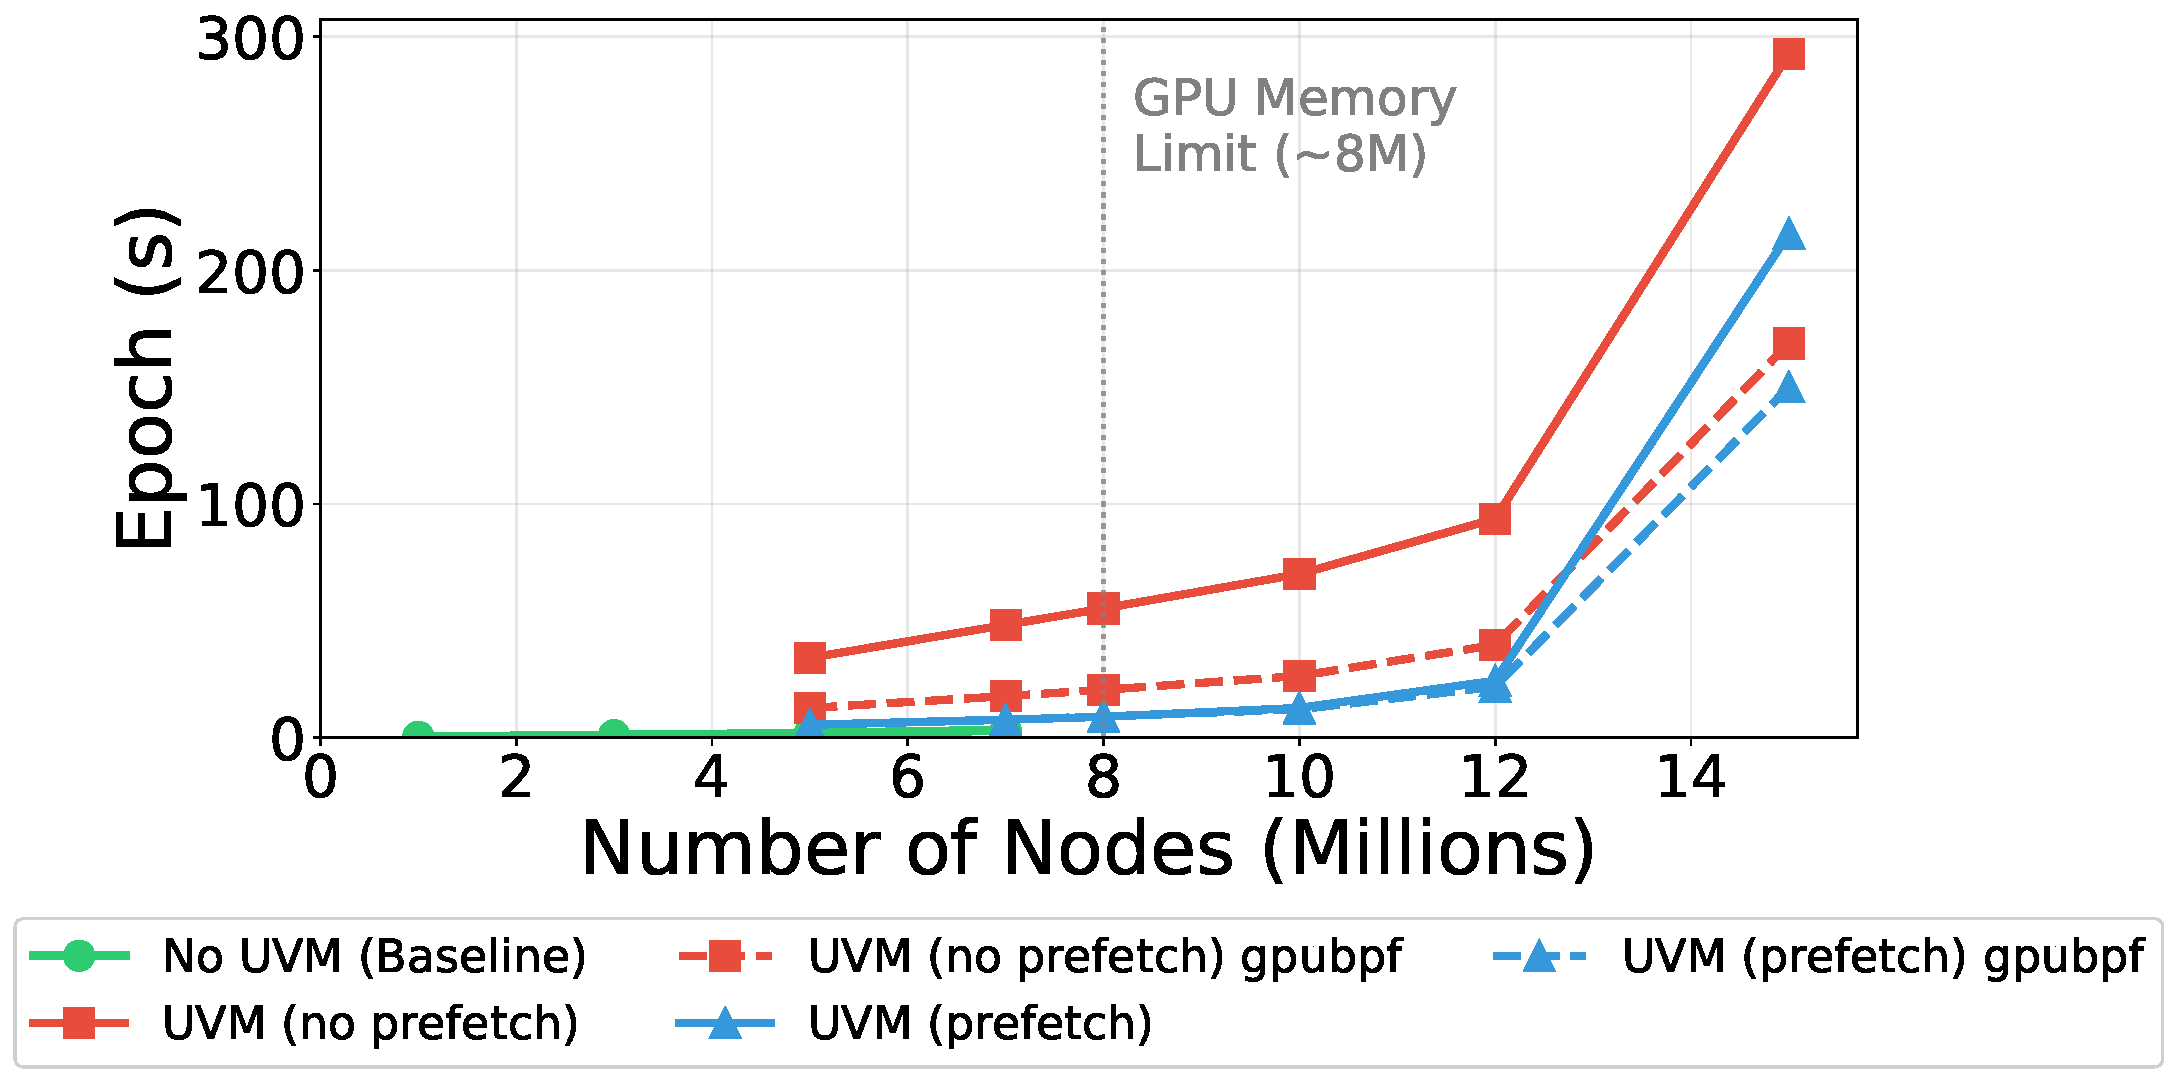
\includegraphics[width=\columnwidth]{img/results-raw/pytorch/uvm_benchmark_comparison.pdf}

\caption{GCN training epoch time vs graph size on PyTorch.}
% PyTorch 上 GCN 训练的单轮时间随图规模的变化。
\label{fig:gnn-epoch}
\end{figure}

\paragraph{Faiss Vector Search.}
% Faiss 向量检索。
We evaluate \sys on vector similarity search using the SIFT dataset with an IVF4096,Flat index, scaling from 20M (9.5GB) to 50M (24GB) and 100M (48GB, exceeding GPU memory).
% 我们使用 SIFT 数据集和 IVF4096,Flat 索引评估向量相似度检索，规模从 20M（9.5GB）到 50M（24GB）再到 100M（48GB，超过 GPU 显存）。
IVF indexes have a two-level structure: frequently-accessed centroids and larger posting lists, and Faiss operations have two distinct phases: BUILD performs sequential scans while SEARCH issues random accesses.
% IVF 索引具有两级结构：被频繁访问的聚类中心和更大的 posting list；Faiss 操作有两个不同阶段：BUILD 执行顺序扫描，SEARCH 发起随机访问。
\sys reduces build time by 21--29\% on 50M, scaling to 27--40\% on 100M as memory pressure grows.
% 在 50M 规模上，gpubpf 将构建时间降低 21--29\%，在 100M 上随内存压力增大扩大到 27--40\%。
For search workloads, \sys reduces latency by 10--16\% across different \texttt{nprobe} settings despite the random access patterns inherent in ANN search.
% 对于检索工作负载，尽管 ANN 检索固有的随机访问模式，gpubpf 在不同 \texttt{nprobe} 设置下仍将延迟降低 10--16\%。
As shown in \Cref{fig:faiss-perf}, the converged policy prefetches posting lists sequentially for oversubscribed datasets and uses stride prediction for K-means iterations during index construction; device-side eBPF programs also trigger prefetching of corresponding posting lists.
% 如 \Cref{fig:faiss-perf} 所示，收敛后的策略对超订数据集顺序预取 posting list，并在索引构建期间对 K-means 迭代使用步长预测；设备端 eBPF 程序还会触发相应 posting list 的预取。

The agent tested 8 policies over 5 iterations.
% 智能体在 5 轮迭代中测试了 8 个策略。
Initially, a momentum-based phase detector with cycle eviction improved BUILD but degraded SEARCH, as forward drift in search queries confused the detector.
% 最初，带周期驱逐的基于动量的阶段检测器改善了 BUILD 但恶化了 SEARCH，因为检索查询的前向漂移迷惑了检测器。
Fixing the classifier revealed eviction policy rather than phase detection controlled performance.
% 修正分类器后发现，控制性能的是驱逐策略而非阶段检测。
Version three, pairing the corrected detector with default eviction, converged.
% 第三个版本将修正后的检测器与默认驱逐配对，收敛成功。
A subsequent fast-path optimization introduced a state-machine bug (policy stuck in SEARCH mode), detected and fixed in one iteration.
% 随后的一项快速路径优化引入了一个状态机缺陷（策略卡在 SEARCH 模式），在一个迭代内被检出并修复。
Only 2 of 8 policies yielded positive results.
% 8 个策略中只有 2 个产生了正面结果。

\begin{figure}
\centering

\includegraphics[width=\columnwidth]{img/results-raw/faiss/faiss_benchmark_results.pdf}

\caption{Faiss index build time and query throughput under oversubscription.}
% 超订条件下 Faiss 索引构建时间与查询吞吐量。
\label{fig:faiss-perf}
\end{figure}

% Across all four case studies, \sys's programmable policies exploit workload structure (experts, KV-cache, graph structure, index layout) that existing UVM and framework-level mechanisms cannot leverage, and the agent's exploration followed a consistent pattern: broad initial policy, failure-driven refinement, and iterative convergence, with eBPF containment ensuring every failed attempt was recovered in seconds rather than requiring driver rebuilds or reboots.

\subsubsection{Multi-Tenant Memory, Bandwidth, and Scheduling}
% 多租户内存、带宽与调度
\label{sec:rq1-mt}

We evaluate \sys on multi-tenant GPU workloads, comparing per-tenant policies against global and framework-managed approaches.
% 我们在多租户 GPU 工作负载上评估 gpubpf，将每租户策略与全局策略和框架管理的方法进行对比。

Compute-bound scheduling results are reported with the XSched and GPREEMPT policy ports in \S\ref{sec:policy-mechanism}.
% 计算密集型调度结果与 XSched 和 GPREEMPT 策略移植一并在 \S\ref{sec:policy-mechanism} 报告。

\paragraph{Memory-bound Priority Differentiation.}
% 内存密集型优先级区分。
We evaluate \sys's memory policies for priority differentiation on \emph{memory-bound} workloads under UVM oversubscription using HotSpot~\cite{che2009rodinia} (spatial locality), GEMM from PolyBench~\cite{grauer2012auto} (compute-intensive, memory-bound under UVM oversubscription), and K-Means~\cite{gu2020uvmbench} (sparse access).
% 我们在 UVM 超订下使用 HotSpot~\cite{che2009rodinia}（空间局部性）、来自 PolyBench~\cite{grauer2012auto} 的 GEMM（计算密集，在 UVM 超订下为内存受限）和 K-Means~\cite{gu2020uvmbench}（稀疏访问），在\emph{内存密集型}工作负载上评估 gpubpf 的内存优先级区分策略。
Each experiment runs two concurrent processes competing for GPU memory.
% 每个实验运行两个并发进程竞争 GPU 内存。
Policy labels use priority values 0--100 (lower = higher priority): \texttt{Prefetch(lo,hi)} prefetches pages for processes in that range, while \texttt{Evict(lo,hi)} selects eviction victims accordingly.
% 策略标签使用 0--100 的优先级数值（数值越低优先级越高）：\texttt{Prefetch(lo,hi)} 为处于该范围的进程预取页面，\texttt{Evict(lo,hi)} 则据此选择驱逐对象。
We compare against no-policy execution and retain single-process runtime (Single~1$\times$) and twice that runtime as sequential references, not proven concurrent lower bounds.
% 我们与无策略执行对比，并保留单进程运行时（Single 1×）及其两倍作为顺序执行参考，而非已证明的并发下界。

The historical single-round records in \Cref{fig:all-kernels-priority}(a--c) show memory-policy completion-time proxies 55--92\% below no-policy execution.
% \Cref{fig:all-kernels-priority}(a--c) 中的历史单轮记录显示，内存策略的完成时间代理指标比无策略执行低 55--92\%。
The recorded scheduler differences below 1\% do not establish ineffectiveness: those runs did not confirm policy engagement or independently timestamp both tenant exits.
% 其中不足 1\% 的调度差异不能证明策略无效：这些运行没有确认策略实际执行，也没有独立记录两个租户的退出时间。
% Retained historical draft number: high-priority processes complete 6--19\% faster; the earlier source and raw records remain in the artifact, without promoting this to an independently timed repeated result.
In the fresh five-block HotSpot comparison in \Cref{fig:all-kernels-priority}(d), high/low process-duration medians are 56.55/56.60 s without policy, 25.16/26.85 s with memory policy, 3.94/6.08 s with timeslicing, and 3.55/6.46 s with both.
% 在 \Cref{fig:all-kernels-priority}(d) 的新五组 HotSpot 对比中，高/低优先级进程耗时中位数为：无策略 56.55/56.60 秒、内存策略 25.16/26.85 秒、时间片策略 3.94/6.08 秒、组合策略 3.55/6.46 秒。
These independently measured durations include initialization, warmup and teardown; every scheduling-bearing run records 12 policy hits and timeslice modifications.
% 这些独立测得的耗时包含初始化、预热和清理；每个包含调度策略的运行均记录了 12 次策略命中和时间片修改。
Adding memory policy to timeslicing reduces high-priority duration by a paired median 10.2\% but increases low-priority duration by 6.3\%: composition exposes a priority tradeoff, not an all-workloads or all-metrics advantage of the mechanism.
% 在时间片策略上叠加内存策略，使高优先级耗时的配对中位数降低 10.2\%，但低优先级耗时增加 6.3\%：组合揭示了优先级取舍，而非机制在所有负载或指标上的优势。
% Evidence: gpu_ext 10994d21; workloads/fig13-fast/results-performance-575-20260907.md. Historical files and sub-1\% observations are retained.

\begin{figure*}[t]
\centering
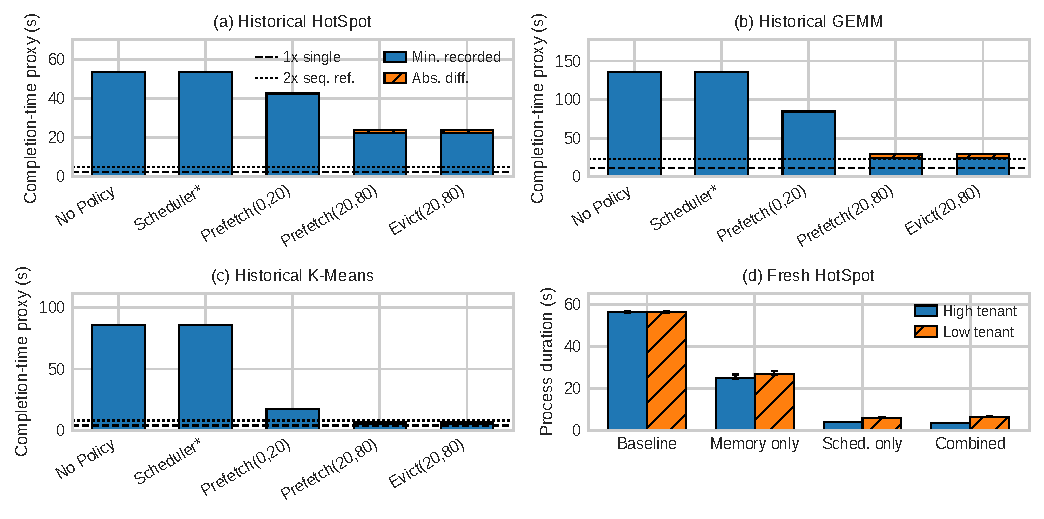
\includegraphics[width=\textwidth]{img/results-raw/multi-tenant/fig13_expanded.pdf}

\caption{Memory and scheduling policies under UVM oversubscription. (a--c) Historical single-round records: stacked minimum and absolute difference of recorded tenant durations give completion-time proxies, not reconstructed overlap. Scheduler* engagement was unconfirmed; 1$\times$ single and 2$\times$ sequential lines are references, not concurrent lower bounds. (d) Fresh HotSpot process durations, measured independently including initialization and warmup: medians and full min--max ranges over five interleaved blocks. Combining memory and scheduling favors the high-priority tenant at a cost to the low-priority tenant.}
% UVM 超订下的内存与调度策略。(a--c) 历史单轮记录：两个租户记录耗时的最小值与绝对差堆叠形成完成时间代理指标，而非重建的重叠时间。Scheduler* 未确认实际执行；单进程及两倍顺序执行虚线仅为参考，并非并发下界。(d) 新 HotSpot 进程耗时，独立测量且包含初始化与预热：五个交错组的中位数及完整最小至最大范围。组合策略以低优先级租户的代价改善高优先级租户。
\label{fig:all-kernels-priority}
\end{figure*}

\paragraph{Two-Tenant: High-Priority LLM Inference + Background Training.}
% 双租户：高优先级 LLM 推理 + 后台训练。
We run two tenants sharing a single GPU: T1 is a high-priority \texttt{llama.cpp} inference service (LC workload) serving 100 ShareGPT prompts at 0.2 RPS, and T2 is a background PyTorch GNN training job (BE workload) with 8M nodes requiring 36GB peak memory (oversubscribed).
% 我们让两个租户共享一块 GPU：T1 是高优先级的 \texttt{llama.cpp} 推理服务（LC 工作负载），以 0.2 RPS 服务 100 条 ShareGPT 提示；T2 是后台的 PyTorch GNN 训练作业（BE 工作负载），8M 节点，峰值内存需求 36GB（超订）。
We compare default UVM (driver FIFO/LRU) against \sys per-tenant memory and scheduler policies (combining Quota LRU, Tree-based Prefetch, and Dynamic Timeslice).
% 我们将默认 UVM（驱动 FIFO/LRU）与 gpubpf 的每租户内存和调度器策略（结合 Quota LRU、基于树的预取和动态时间片）进行对比。
\Cref{fig:two-tenant} shows mutual improvement: LC TPOT drops by 40--45\% and TTFT by 14--20\%, while GNN training simultaneously improves by 28\%, approaching the ideal fair share baseline.
% \Cref{fig:two-tenant} 显示双方同时受益：LC 的 TPOT 下降 40--45\%，TTFT 下降 14--20\%，同时 GNN 训练也改善 28\%，接近理想的公平份额基线。
This shows \sys reduces contention for both workloads rather than favoring one over the other.
% 这说明 gpubpf 减轻了两种工作负载之间的竞争，而非偏袒其中一方。

Our multi-tenant setting is software co-location on an unpartitioned GPU, complementary to static partitioning: SemiAnalysis's critique~\cite{semianalysis2025partitioning} targets fixed MIG subdevices for large-model inference, not software policies that rebalance resources at runtime.
% 我们的多租户场景是未分区 GPU 上的软件共置，与静态分区互补：SemiAnalysis 的批评~\cite{semianalysis2025partitioning} 针对的是大模型推理下固定的 MIG 子设备，而非运行时动态再平衡资源的软件策略。

\begin{figure}
\centering

\includegraphics[width=\columnwidth]{img/results-raw/multi-tenant/fig_colocated_results.pdf}

\caption{Two-tenant co-location: \texttt{llama.cpp} inference (LC) + GNN training (BE).}
% 双租户共置：\texttt{llama.cpp} 推理（LC）+ GNN 训练（BE）。
\label{fig:two-tenant}

\end{figure}

\begin{figure*}[!t]
\centering

\includegraphics[width=\textwidth]{img/results-raw/runtime/microbench_comparison.pdf}
\caption{Device-side overhead. (a) Naive per-thread injection vs \sys's SIMT-aware execution. (b) CPU map access latency via PCIe vs GPU-side operations.}
% 设备端开销。(a) 朴素的每线程注入与 gpubpf 的 SIMT 感知执行对比。(b) 经 PCIe 的 CPU map 访问延迟与 GPU 端操作对比。
\label{fig:microbench}
\end{figure*}

\subsubsection{Policy Expressibility and Matched Implementations}
% 策略可表达性与匹配实现
\label{sec:policy-mechanism}

We evaluate whether \sys{} can express the policies of published state-of-the-art systems, and what the general mechanism costs when it runs the same policy as an ad-hoc implementation.
% 我们评估 \sys{} 能否表达已发表最先进系统的策略，以及通用机制在运行与临时实现相同的策略时代价几何。
\Cref{fig:matched-ports} separates two comparisons: a workload baseline versus a native policy implementation measures policy benefit, while native versus \sys{} on the same executor measures the port's cost; XSched and GPREEMPT appear in \Cref{fig:scheduler-latency}.
% \Cref{fig:matched-ports} 区分两层比较：工作负载基线与原生策略实现比较策略收益，相同执行器上的原生实现与 \sys{} 比较移植代价；XSched 和 GPREEMPT 见 \Cref{fig:scheduler-latency}。
The ports span host-side expert caching and queue admission, driver-side timeslicing and memory migration, and device-side task selection.
% 这些移植覆盖主机侧的专家缓存与队列准入、驱动侧的时间片与内存迁移，以及设备侧的任务选择。

\begin{figure*}[t]
\centering
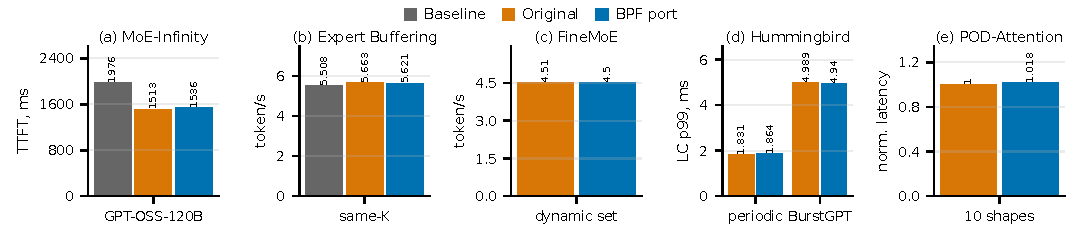
\includegraphics[width=\textwidth]{img/results-raw/revision/matched-port-panels.pdf}
\caption{Matched policy ports on RTX~5090. Baselines are (a) prediction-disabled expert caching, (b) fixed-$K$ FIFO, (c) all-positive prefetch, (d) default scheduling, and (e) two-stream FlashAttention. Each panel reports one metric over five blocks: median first-visible-text latency (a), median throughput (b,c), median LC response p99 (d), and mean operator latency for Llama decode batch 128 (e). Native-policy bars use the same executor as \sys{}; panel (d) uses the idle-admission component.}
% RTX~5090 上的匹配策略移植。基线依次为关闭预测的专家缓存、固定 K 的 FIFO、全正例预取、默认调度和双流 FlashAttention。每个面板报告五组实验中的一个指标：首个可见文本延迟中位数（a）、吞吐中位数（b、c）、LC 响应 p99 中位数（d），以及 Llama 解码批量 128 的平均算子延迟（e）。原生策略与 \sys{} 使用相同执行器；面板（d）使用空闲准入组件。
\label{fig:matched-ports}
\end{figure*}

\paragraph{Methodology}
% 方法
Each comparison pairs a native implementation with a \sys{} port of the same policy on the same workload and executor, on RTX~5090 (driver 575.57.08) with exclusive GPU access and repeated randomized trials.
% 每组对比在相同工作负载和执行器上，将原生实现与同一策略的 \sys{} 移植版配对，在 RTX~5090（驱动 575.57.08）上以独占 GPU 和重复随机试验运行。
Unless stated otherwise, we report medians with paired bootstrap intervals; POD's operator plot uses the mean of five per-run means.
% 除非另有说明，我们报告中位数及配对 bootstrap 区间；POD 算子图使用五次运行均值的平均值。

\paragraph{MoE-Infinity (expert offloading)}
% MoE-Infinity（专家卸载）
Host-JIT \sys{} programs implement MoE-Infinity's~\cite{xue2025moeinfinity} prediction matching, prefetch ranking, and eviction selection, while the shared GPT-OSS-120B executor performs expert transfers and inference.
% 主机 JIT 的 \sys{} 程序实现 MoE-Infinity~\cite{xue2025moeinfinity} 的预测匹配、预取排序和驱逐选择，共用的 GPT-OSS-120B 执行器负责专家传输与推理。
Across five paired runs, the native policy and \sys{} reduce first-visible-text latency by 22.1\% and 22.5\%, respectively, relative to prediction-disabled expert caching.
% 五次配对试验中，相对关闭预测的专家缓存，原生策略与 \sys{} 分别将首个可见文本延迟降低 22.1\% 和 22.5\%。

\paragraph{XSched (preemptive scheduling)}
% XSched（抢占式调度）
We port XSched's~\cite{shen2025xsched} inter-kernel preemption: a host-JIT \sys{} program selects the highest-priority task, and the original executor performs suspend/resume.
% 我们移植 XSched~\cite{shen2025xsched} 的内核间抢占：主机 JIT 的 \sys{} 程序选择最高优先级任务，原始执行器执行挂起/恢复。
With two latency-critical (LC) and four best-effort (BE) processes, LC submission-to-first-CTA p99 falls from 76.9~s under native CUDA to 27.0~s with XSched and 27.3~s with \sys{} (\Cref{fig:matched-scheduling}).
% 在两个延迟关键（LC）和四个尽力型（BE）进程下，LC 提交到首个 CTA 的 p99 从原生 CUDA 的 76.9 秒降至 XSched 的 27.0 秒和 \sys{} 的 27.3 秒（\Cref{fig:matched-scheduling}）。

\paragraph{GPREEMPT (priority timeslicing)}
% GPREEMPT（优先级时间片）
For GPREEMPT~\cite{fan2025gpreempt}, host-JIT \sys{} programs issue blocking and release decisions, and kernel-BPF programs assign priority-based timeslices; the original executor and GPU driver carry out these decisions.
% 对 GPREEMPT~\cite{fan2025gpreempt}，主机 JIT 的 \sys{} 程序做出阻塞与释放决策，内核 BPF 程序按优先级分配时间片，由原始执行器和 GPU 驱动执行。
Under continuous background load, this policy reduces LC response p99 from 1.796~ms under default scheduling to 1.615~ms with the original C policy and 1.610~ms with \sys{} (\Cref{fig:matched-scheduling}).
% 在连续后台负载下，GPREEMPT~\cite{fan2025gpreempt} 的优先级时间片将 LC 响应 p99 从默认调度的 1.796 毫秒降至原始 C 策略的 1.615 毫秒和 \sys{} 的 1.610 毫秒（\Cref{fig:matched-scheduling}）。

\begin{figure}
\centering
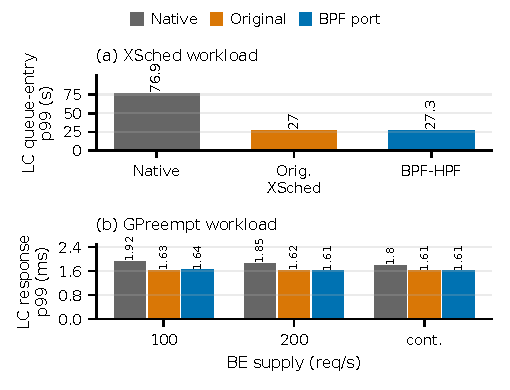
\includegraphics[width=\columnwidth]{img/results-raw/revision/scheduling-comparison-lc-bars.pdf}

\caption{Matched scheduling policies on RTX~5090, LC latency: (a) XSched workload, two LC and four BE processes, LC queue-entry p99; (b) VGG19 LC at 100 requests/s against three ResNet152 BE loads, arrival-to-verified-response p99. Bars show medians (XSched: ten paired repetitions; GPreempt: five per load).}
% RTX 5090 上的匹配调度策略，LC 延迟：(a) XSched 工作负载，两个 LC 和四个 BE 进程，LC 入队 p99；(b) VGG19 LC 每秒 100 请求、对应三种 ResNet152 BE 负载，到已验证响应的 p99。柱形为中位数（XSched：十次配对重复；GPreempt：每种负载五次）。
\label{fig:scheduler-latency}
\label{fig:matched-scheduling}
\end{figure}

\paragraph{Expert Buffering (expert residency)}
% Expert Buffering（专家驻留）
A host-JIT \sys{} program implements Expert Buffering's~\cite{huang2023towards} inactive-first expert admission and eviction decisions, which the shared cache executor applies.
% 主机 JIT 的 \sys{} 程序实现 Expert Buffering~\cite{huang2023towards} 非活跃优先的专家准入与驱逐决策，由共用的缓存执行器执行。
Throughput improves over fixed-$K$ FIFO by 2.6\% with the native policy and 1.8\% with \sys{}.
% 相比固定 K 的 FIFO，原生策略与 \sys{} 分别将吞吐提高 2.6\% 和 1.8\%。

\paragraph{FineMoE (dynamic expert sets)}
% FineMoE（动态专家集）
A host-JIT \sys{} program implements FineMoE's~\cite{yu2026finemoe} dynamic-set rule to select experts for speculative prefetch, while the shared inference executor performs their transfers and computation.
% 主机 JIT 的 \sys{} 程序实现 FineMoE~\cite{yu2026finemoe} 的动态集合规则，选择推测预取的专家，由共用的推理执行器完成传输与计算。
\sys{} improves throughput by 24.6\% over an all-positive prefetch policy that fetches every positive prediction; native and \sys{} throughput differ by 0.21\% in paired runs (95\% CI $[-0.17\%,+0.52\%]$).
% 对 FineMoE~\cite{yu2026finemoe} 的动态专家集选择，相比预取所有正预测的全正例策略，\sys{} 将吞吐提高 24.6\%；原生与 \sys{} 在配对运行中的吞吐差异为 0.21\%（95\% CI $[-0.17\%,+0.52\%]$）。
However, disabling speculative prefetch remains faster: demand-only/native/\sys{} throughput medians are 5.17/4.50/4.51 token/s, and \sys{} is 12.6\% slower than demand-only in paired runs; the gain over all-positive does not establish a net benefit from speculation on this workload.
% 但关闭推测预取仍更快：仅按需加载/原生/\sys{} 的吞吐中位数为 5.17/4.50/4.51 token/s，\sys{} 在配对运行中比仅按需加载慢 12.6\%；优于全正例消融不代表推测预取在此负载上有净收益。
% Evidence: gpu_ext workloads/finemoe/results-performance.md, all 20 completed cells retained; no rerun.

\paragraph{Hummingbird (idle admission)}
% Hummingbird（空闲准入）
A host-JIT \sys{} program implements Hummingbird's~\cite{hu2026hummingbird} idle-admission rule by deciding when background work may enter a foreground idle interval, while the shared DNN executor submits the admitted work.
% 主机 JIT 的 \sys{} 程序实现 Hummingbird~\cite{hu2026hummingbird} 的空闲准入规则，决定后台工作何时可进入前台空闲区间，由共用的 DNN 执行器提交获准的工作。
Across periodic and BurstGPT arrivals, \sys{} lowers LC response p99 by 5.9--9.1\% relative to default scheduling, compared with 7.5--8.2\% for C.
% 在周期性和 BurstGPT 到达模式下，相对默认调度，\sys{} 将 LC 响应 p99 降低 5.9--9.1\%，C 实现降低 7.5--8.2\%。
Both ports pay for this foreground protection with background throughput: BE goodput medians fall from 179.2333/179.1500 req/s under native CUDA admission to 133.2167/133.1667 req/s with the C port and 133.0500/132.8167 req/s with the BPF port under periodic/BurstGPT arrivals.
% 两个移植以前台保护换取后台吞吐：周期/BurstGPT 到达下，BE 良吞吐中位数从原生 CUDA 准入的 179.2333/179.1500 req/s 降至 C 移植的 133.2167/133.1667 req/s 与 BPF 移植的 133.0500/132.8167 req/s。
Relative to fixed GPreempt admission, both ports lose about 19--20\% of this goodput in paired comparisons, a foreground/background tradeoff of this conservative compatibility port on the GPreempt DNN frontend rather than a measured property of the original Hummingbird scheduling policy.
% 相对固定 GPreempt 准入，两个移植在配对比较中损失约 19--20\% 的该良吞吐；此前台/后台权衡描述的是 GPreempt DNN 前端上保守兼容移植的属性，而非实测的原版 Hummingbird 调度策略属性。
% Evidence: workloads/hummingbird/results-575-20260903.md; all 50 cells accepted; no rerun.

\paragraph{POD-Attention (device-side selection)}
% POD-Attention（设备端选择）
A device-side \sys{} program implements POD-Attention's~\cite{kamath2025pod} proportional selection of prefill or decode work for each SM, which the fused attention kernel executes.
% 设备端 \sys{} 程序实现 POD-Attention~\cite{kamath2025pod} 按比例为每个 SM 选择 prefill 或 decode 工作的策略，由融合注意力内核执行。
We evaluate ten shapes over five blocks against non-fused FlashAttention and native POD implementations.
% 我们在十种形状和五组实验中与未融合的 FlashAttention 及原生 POD 实现比较。
For Llama decode batch 128, operator latency falls from 5.360~ms with two-stream FlashAttention to 4.322~ms with the CUDA selector and 4.344~ms with \sys{}.
% 在 Llama 解码批量 128 下，算子延迟从双流 FlashAttention 的 5.360 毫秒降至 CUDA 选择器的 4.322 毫秒和 \sys{} 的 4.344 毫秒。

\paragraph{Mechanism cost}
% 机制代价
The matched comparisons separate policy benefit from the cost of executing the same decisions through \sys{}.
% 匹配对比区分策略收益与通过 \sys{} 执行相同决策的代价。
These costs are operation-specific examples from particular workloads and hooks rather than a universal overhead bound: Expert Buffering incurs 0.7\% overhead; POD's paired operator-latency effects range from a 0.44\% reduction to a 1.18\% increase across ten shapes; a kernel-verified UVM no-prefetch policy incurs 3.2\% overhead over fifteen paired fault-path runs.
% 这些代价是特定工作负载与钩子下的操作级示例，而非通用的开销界限：Expert Buffering 的开销为 0.7\%；POD 在十种形状上的配对算子延迟效应从降低 0.44\% 到增加 1.18\%；经内核验证的 UVM 无预取策略在十五次配对缺页路径运行中的开销为 3.2\%。
Storage measurements also limit this attribution: BPF/native paired p99 differences in the LMCache port (\S\ref{sec:rq1-agent}) range from $-39.7\%$ to $+33.8\%$ across five blocks of the same workload, so this variability precludes a tight estimate of mechanism overhead.
% 存储测量也限制了这种归因：在 LMCache 移植（\S\ref{sec:rq1-agent}）的同一工作负载五个组内，BPF 相对原生的配对 p99 差异从 -39.7\% 到 +33.8\%，这种变动使得机制开销无法得到精确估计。

\paragraph{Agent-discovered policies}
% 智能体发现的策略
Beyond reproducing published policies, our study also included agent-discovered combinations of cross-layer observations and controls.
% 除了复现已发表的策略，我们的研究还包含智能体发现的跨层观测与控制组合。
In the MoE study (\S\ref{sec:eval}), device-side tracing led the agent to a stride-prefetch policy aligned with per-layer expert weight layout combined with LFU eviction that protects shared layers; in the KV-cache study, the agent differentiated prefetch by region type (stride for weights, sequential for KV-cache) under a PCIe-utilization budget, avoiding the mutual thrashing that a uniform policy causes.
% 在 MoE 研究（\S\ref{sec:eval}）中，设备端追踪引导智能体得出与每层专家权重布局对齐的步长预取策略，并结合保护共享层的 LFU 驱逐；在 KV-cache 研究中，智能体在 PCIe 利用率预算下按区域类型区分预取（权重用步长、KV-cache 用顺序），避免了统一策略导致的相互抖动。
Both combinations couple device-side observation with host-side action---device-traced access patterns driving host-side cache and migration decisions---and share the tradeoff that migration spends transfer bandwidth that demand traffic also needs.
% 两种组合都将设备端观测与主机端动作耦合——由设备端追踪到的访问模式驱动主机端的缓存与迁移决策——并共有一个权衡：迁移会占用需求流量所需的传输带宽。
Other systems may implement similar algorithms, but they would need their own observation and enforcement integration to couple device-side observations with migration and admission controls.
% 其他系统可以实现类似的算法，但需要自身的观测与执行集成，才能将设备端观测与迁移和准入控制耦合起来。

\subsection{RQ2: Mechanism Cost}
% RQ2：机制代价
\label{sec:rq2-cost}

We measure hook, observability, and map-placement overheads below; \S\ref{sec:policy-mechanism} reports the execution costs of matched policy ports.
% 下文测量钩子、可观测性和 map 放置开销；\S\ref{sec:policy-mechanism} 报告匹配策略移植的执行代价。

\paragraph{Verification Overhead.}
% 验证开销。
Load-time verification takes 141~ms for \texttt{kernelretsnoop} and 12~ms for \texttt{threadhist}; steady-state throughput with strict verification is statistically indistinguishable from unverified execution for both tools.
% 加载时验证对 \texttt{kernelretsnoop} 耗时 141~ms，对 \texttt{threadhist} 耗时 12~ms；两个工具在严格验证下的稳态吞吐量与未验证执行在统计上不可区分。

\paragraph{Host Runtime Overhead.}
% 主机运行时开销。
We quantify the overhead of the \sys driver runtime independent of policy logic using GEMM from PolyBench~\cite{grauer2012auto} and HotSpot~\cite{che2009rodinia} (1.1$\times$ oversubscription, 35~GB working set) on RTX 5090.
% 我们使用 PolyBench~\cite{grauer2012auto} 的 GEMM 和 HotSpot~\cite{che2009rodinia}（1.1× 超订、35 GB 工作集）在 RTX 5090 上量化 gpubpf 驱动运行时独立于策略逻辑的开销。
With hooks enabled but no policy attached, the overhead is less than 0.2\%.
% 启用钩子但不附加策略时，开销小于 0.2\%。

\paragraph{Device-side Overhead.}
% 设备端开销。
We evaluate device-side observability tools built on \sys (\Cref{fig:obs-overhead}) using llama.cpp prefill on two GPUs: the P40 (Llama 1B, sequence-mixed) and the RTX~5090 (TinyLlama-1.1B, ten randomized repetitions with paired custom NVBit adapters~\cite{villa2019nvbit}).
% 我们在两块 GPU 上使用 llama.cpp 预填充评估基于 gpubpf 构建的设备端可观测工具（\Cref{fig:obs-overhead}）：P40（Llama 1B，序列混合）和 RTX~5090（TinyLlama-1.1B，十次随机重复，配对的定制 NVBit 适配器~\cite{villa2019nvbit}）。
Tools include \texttt{kernel\-ret\-snoop} (per-block finish timestamps), \texttt{thread\-hist} (load imbalance detection), and \texttt{launch\-late} (GPU kernel launch latency).
% 工具包括 \texttt{kernel\-ret\-snoop}（每块完成时间戳）、\texttt{thread\-hist}（负载不均衡检测）和 \texttt{launch\-late}（GPU 内核启动延迟）。
Overhead is measured as token/s degradation during prefill.
% 开销以预填充期间 token/s 的下降来衡量。
On the P40, \sys achieves 3--14\% overhead versus NVBit's 85--93\%, due to the warp-uniform execution model.
% 在 P40 上，得益于 warp 统一执行模型，gpubpf 的开销为 3--14\%，而 NVBit 为 85--93\%。
On the RTX~5090, \sys has lower overhead than NVBit for all three tools: 90.71\% versus 99.62\% for the complete per-warp kernel-return stream, 2.97\% versus 10.35\% for the exit-count histogram, and 0.22\% versus 8.80\% for \texttt{launchlate}. The full record stream remains expensive even with warp-level recording.
% 在 RTX~5090 上，gpubpf 在三个工具上的开销均低于 NVBit：完整的逐 warp 内核返回记录流为 90.71\% 对 99.62\%，退出计数直方图为 2.97\% 对 10.35\%，\texttt{launchlate} 为 0.22\% 对 8.80\%。即使按 warp 记录，完整记录流的开销仍然很高。
A separate five-pair experiment buffers the complete kernel-return records in a GPU-local array, yielding mean prefill overhead of 5.57\% (range 4.02--6.70\%) while retaining all 720,896 records per run.
% 另一组五次配对实验将完整的内核返回记录缓存在 GPU 本地数组中，平均预填充开销为 5.57\%（范围 4.02--6.70\%），每次运行保留全部 720,896 条记录。
The final 23.2~MB readback averages 10.38~ms outside prefill timing; the finite buffer is sized for this pp512, serial-launch workload, not unbounded streaming.
% 最终 23.2~MB 回读平均耗时 10.38~ms，不计入预填充计时；该有限缓冲区按本次 pp512、串行启动工作负载配置，并非无界流式记录。
Like the RTX~5090 tool campaign, this variant uses warning-mode admission and provides performance evidence, not evidence of strict verifier acceptance.
% 与 RTX~5090 工具实验相同，该变体使用警告模式准入，提供性能证据，而非严格验证器接受该程序的证据。
Attaching to a running process requires no application restart.
% 附加到正在运行的进程无需重启应用。

\begin{figure}[t]
\centering
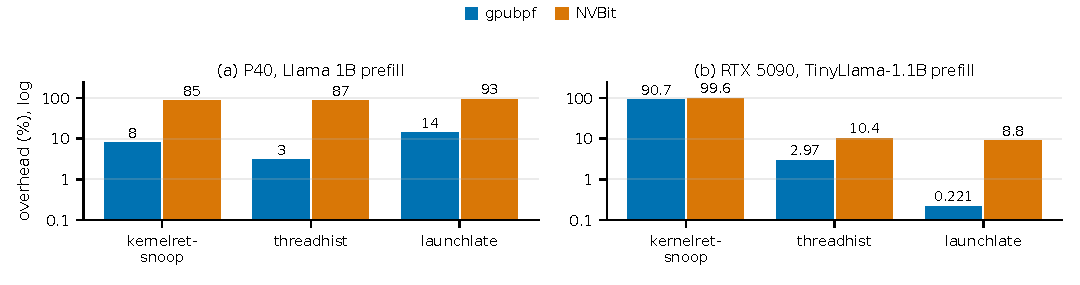
\includegraphics[width=\columnwidth]{img/results-raw/revision/obs-overhead-bars.pdf}
\caption{\sys device-side observability overhead versus NVBit (log scale). (a) P40, Llama 1B. (b) RTX~5090, TinyLlama-1.1B, ten paired runs.}
% gpubpf 设备端可观测开销与 NVBit 对比（对数坐标）。(a) P40，Llama 1B。(b) RTX~5090，TinyLlama-1.1B，十次配对运行。
\label{fig:obs-overhead}
\end{figure}

\paragraph{Device-side Runtime Optimization.}
% 设备端运行时优化。
We evaluate device-side \sys mechanisms using a vector-add CUDA GPU kernel (32 elements, 10K iterations) from cuda-sample~\cite{nvidia_cuda_samples} on RTX 5090.
% 我们使用来自 cuda-sample~\cite{nvidia_cuda_samples} 的 vector-add CUDA GPU 内核（32 个元素、10K 次迭代）在 RTX 5090 上评估 gpubpf 的设备端机制。
\Cref{fig:microbench}(a) compares \sys's SIMT-aware warp-level execution against eGPU~\cite{egpu} that injects eBPF bytecode without SIMT-specific verification and optimizations.
% \Cref{fig:microbench}(a) 将 gpubpf 的 SIMT 感知 warp 级执行与 eGPU~\cite{egpu} 对比，后者注入 eBPF 字节码而不进行面向 SIMT 的验证与优化。
The baseline incurs overhead due to per-thread execution and uncoalesced memory access, while \sys's warp-uniform execution and coalesced map access reduce overhead by 60--80\%.
% 基线因每线程执行和未合并的内存访问产生开销，而 gpubpf 的 warp 统一执行与合并 map 访问将开销降低 60--80\%。
\Cref{fig:microbench}(b) compares CPU map access via PCIe against GPU-side operations, motivating \sys's hierarchical map design that keeps hot state on GPU.
% \Cref{fig:microbench}(b) 对比了经 PCIe 的 CPU map 访问与 GPU 端操作，这促使 gpubpf 采用将热状态保留在 GPU 上的分层 map 设计。
We do not compare policy-level performance against the prior workshop version or Neutrino because they are limited to read-only observability (\S\ref{sec:background}). %\arq{Do we need this experimentation?  I guess you're wanting to show that this current version of the system is better than the workshop version, but I wonder if that is entirely surprising.}
% 我们不在策略层面与先前的工作坊版本或 Neutrino 比较，因为它们仅限于只读可观测性（\S\ref{sec:background}）。
